\subsection{Activation Image Summaries}

\todo{maybe refer to this as ``Layer Summarization''?}

\begin{figure}[b]
\centering
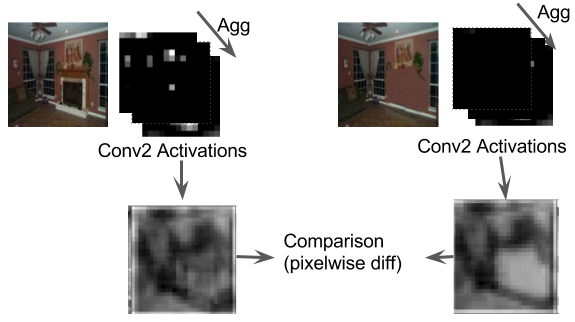
\includegraphics[width=\columnwidth]{figures/activation_image_summary_fig}
\caption{Generation of Activation Image Summaries for Comparison}
\label{fig:act_im_summary_fig}
\end{figure}

We define an activation image summary as an pixel by pixel aggregation over the activations images in a layer of a CNN. For instance, the conv4 layer of Alexnet~\cite{alexnet} contains 256 distinct $14 \times 14$ activation images. We generate an activation image summary by aggregating over each pixel across the set of activation images in a layer. In Activation image summaries are particularly useful for comparing the activations of an image and the same image perturbed in some way. Comparing the layer-by-layer summaries of an original and a perturbed image reveals changes in the overall activations in a layer that may lead to change in activations. The process of generating summaries and comparing them for an original image and a perturbed image is demonstrated in figure ~\ref{fig:act_im_summary_fig} where the aggregation function is a simple average over the pixels of the activation images of a correctly classified living room image and the same image with the fireplace removed by image manipulation software. We hypothesize that for a perturbed image, where the change in the image should not change the output class, that 

The choice of aggregation function for the summary has a direct impact on the type of knowledge gained from activation summary images. 